%\section{CSO as sources of UHECRs and neutrinos}
\label{sec:CSO_UHECR}
Following the new definition of CSO and the new morphology they undergo, it becomes interesting to study if they are a candidate for the acceleration of UHECRs and neutrinos. This section will estimate several parameters of their structure and explore the possibility of CSOs as sources of UHECRs and neutrinos. 

\section{Parameter estimation}
\subsection{Magnetic field strength}


In order to estimate magnetic field strength, we outlined two methods in section \ref{sec:equipartition} and \ref{sec:SSA}. Both values will work as great cross-checks for eachother because of different proportionality where $B \propto R^{4}$ for SSA, and $B \propto R^{-6/7}$ for equipartition.


The data we need to estimate both methods is not all in the orignal table of CSOs. Therefore, we will estimate both method for sources that have entries in two catalogues, The first is the catalogue by \cite{kiehlmann2023compact} given in Table \ref{tab:CSO_sources} and the second is the catalouge of radio observation from the VLBA at 5GHz called The VSOP 5 GHz Continuum Survey: The Pre-launch VLBA Observations, found in \cite{nrao1996}. We find an overlap of $10$ sources between the two catalogues, and the extracted values can be found in table \ref{tab:CSO_B}. The desired parameters are the turnover frequency, the flux density at the turnover frequency, the flux density at $5$GHz, the size of the hotspot, and class. From table \ref{tab:CSO_sources} we are given the turnover frequency and its corresponding flux density. The problem here is that this value is for the entire source and not any hotspot or lobe. In order to derive the appropriate value for only one hotspot, we need to know the size of the hotspot, and importantly the fraction of emitted radiation that stems from that hotspot compared to the rest of the source. In order to determine the size of the hotspot we will turn to the NRAO catalogue, which gives high resolution images and flux densities of the sources and its components at $5$GHz. These images will allow us to estimate the size of an individual lobe through the use of the FWHM as explained in section \ref{sec:size_estimation}. CSO usually have two lobes with two hotspots, and we chose the most powerful hotspot, and calculate the fraction of the total flux density that comes from it. The same fraction will then be applied to the turnover flux density given in table \ref{tab:CSO_sources} to estimate the turnover flux density from this hotspot. Lastly, the NRAO catalogue also gives flux densities measured at $5$GHz at each lobe, allowing us to estimate the equipartition magnetic field strength based on an assumption of the spectral index. From here we can estimate the magnetic fields via both methods and the results can be seen in Figure \ref{fig:B_field} and \ref{fig:B_field_SSA}.






\begin{table}
    \centering
    \begin{tabular}{|c|c|c|c|c|c|c|c|}
    \hline
    \textbf{Name} & \textbf{z} & \textbf{Class} & \textbf{$\nu_t$} & \textbf{$S_{\nu_t}$} & \textbf{$\nu_{5GHz}$} & \textbf{$\theta_{lobe}$} & \textbf{$S_{\nu_{5GHz}}$} \\
    \hline
    J0029+345 & 0.517 & 2.0 & 0.8 & 1.178 & 5 & 2.1 & 0.766 \\
    J0111+3906 & 0.66847 & 2.0 & 4.0 & 0.88189 & 5 & 0.95 & 0.862 \\
    J0119+3210 & 0.0602 & 2.2 & 0.4 & 0.5125 & 5 & 9.85 & 0.205 \\
    J0405+3803 & 0.055 & 2.0 & 0.07 & 2.554 & 5 & 2.7 & 0.418 \\
    J0713+4349 & 0.518 & 2.0 & 1.9 & 0.94311 & 5 & 1.45 & 0.722 \\
    J1035+5628 & 0.0460 & 2.0 & 1.3 & 1.0659 & 5 & 1.6 & 0.741 \\
    J1158+2450 & 0.203 & 2.2 & 2 & 0.588 & 5 & 4 & 0.566 \\
    J1347+1217 & 0.121 & 2.2 & 0.4 & 1.3947 & 5 & 1 & 0.488 \\
    J1407+2827 & 0.077 & 2.1 & 4.9 & 2.9375 & 5 & 1.2 & 2.350 \\
    J2022+6136 & 0.2266 & 2.1 & 4.086 & 1.57256 & 5 & 2 & 1.787 \\
    J2355+4950 & 0.238 & 2.2 & 0.7 & 1.5450 & 5 & 1.8 & 0.791 \\
    \hline
    \end{tabular}
    \caption{Overlapping sources between the NRAO catalogue and \cite{kiehlmann2023compact} and the extracted values scaled to represent one lobe hotspot.}
    \label{tab:CSO_B}
\end{table}


\begin{figure}[H]
    
    \centering
    \begin{subfigure}[b]{0.49\textwidth}
        \centering
        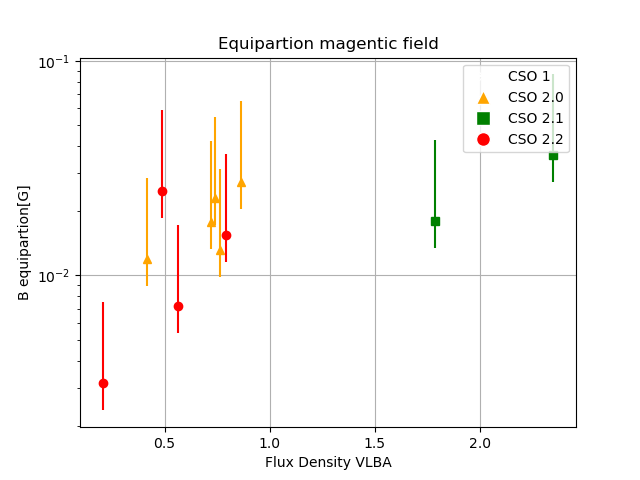
\includegraphics[width=\textwidth]{C:/Users/henri/OneDrive/Documents/NTNU/Semester 10/Masteroppgave/Plots/Equipartion.png}
        \caption{Magnetic field strength estimated from the equipartition method. The errorbars are calculated from the span of values obtained from different spectral index ranging from $0.6$ to $1.3$.}
       
        \label{fig:B_field}
    \end{subfigure}
    \hfill
    \begin{subfigure}[b]{0.49\textwidth}
        \centering
        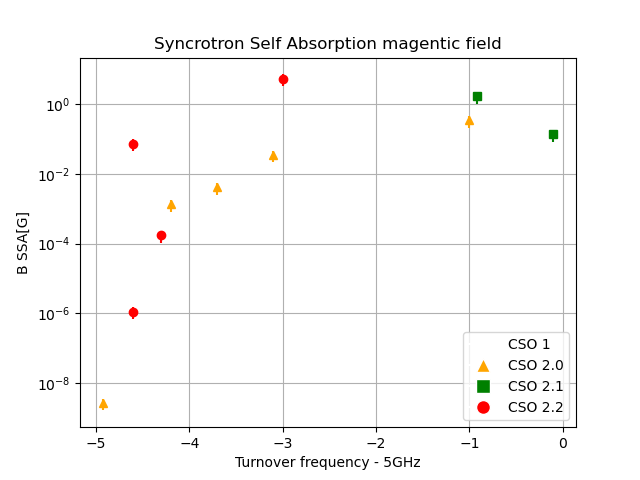
\includegraphics[width=\textwidth]{C:/Users/henri/OneDrive/Documents/NTNU/Semester 10/Masteroppgave/Plots/SSA.png}
        \caption{Magnetic field strength estimated from the SSA method. The errorbars are calculated from the span of values of $b(\alpha)$ obtained from different optical thickness. $b(\alpha)$ ranges from $1.08$ to $2.38$.}
        \label{fig:B_field_SSA}
    \end{subfigure}
\end{figure}





The result of the magnetic field estimations is a little varied, but  most  numbers indicate a magnetic field strength between $ 10^{-2}$ and $1$ G but most are $<10^{-1}$. Here, we rely most heavily on the equipartition argument due to the SSA estimation being quite biased. For example the estimation of the lobe size is most likely wrong for turnover frequencies lower than the imaging. The lobe size estimation is based on the images from the $5$ GHz survey, and from previous papers such as \cite{Marr_2013} who did multifrequency radio imaging, the size of the source via the FWHM method will increase when imaging lower frequencies. In figure \ref{fig:B_field_SSA}, the magnetic field strength from SSA calculations is heavily dependent on the turnover frequency with the lowest values giving unreasonably low numbers. The SSA still gives values for the magnetic field strength that are in the same order of magnitude as the equipartition method at turnover frequencies closer to the measured frequency and even go above.

The SSA estimation still has more caveats than its counterparts, where the most important is the thought that all regions of the AGN radio image, that is the core and its two lobes have the same turnover frequency. Given both lobes have similar morphology we could expect them to have similar turnover frequencies, but the core is a different story. Therefore, the proper estimation of hotspot turnover frequencies can boost the SSA results. In addtion, it could be that there are other factors than synchrotron self-absorption that make the source optically dense. If we include free-free absorption, it would shift the turnover frequency to a higher value, resulting in a higher magnetic field measurement. This is not investigated in this work but is a possible explanation for the higher magnetic field strength compared with $B_{\text{eq}}$. Lastly, the way we calculated the fraction of lobeflux to total flux can also be a source of error. The fractional flux was based on the flux at $5$ GHz, but the true distribution of flux could be different at other frequencies. Here direct measruements at or close to the correct turnover freqeuncy would remove this error.  Even though the SSA method has a lot of caveats its measurments of the magnetic field strength are still reasonable, especially for turnover frequencies that were close to the observed frequencies.

\begin{figure}
    \centering
    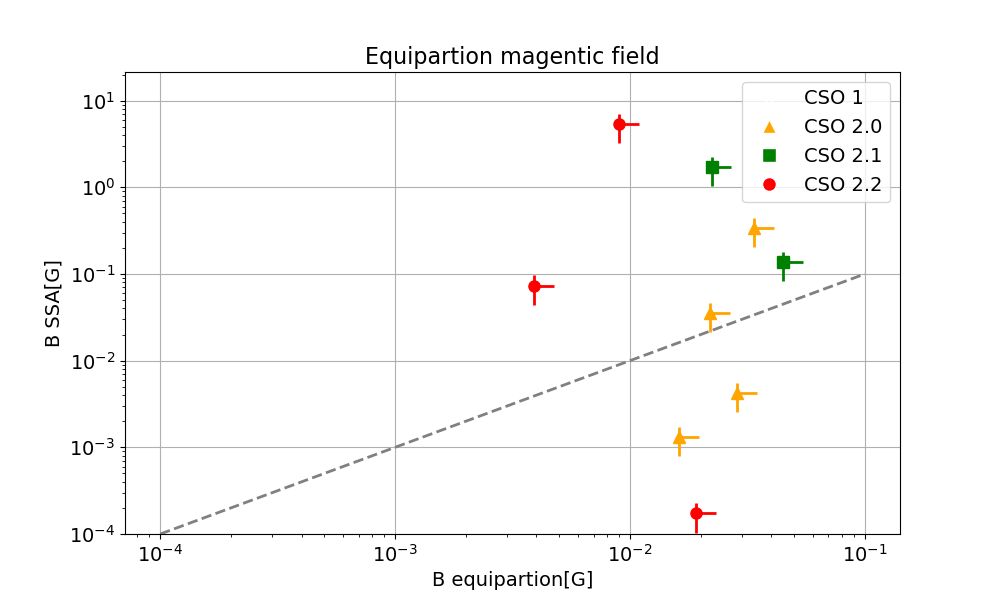
\includegraphics[width=0.8\textwidth]{C:/Users/henri/OneDrive/Documents/NTNU/Semester 10/Masteroppgave/Plots/Equipartion_and_SSA.png}
    \caption{Magnetic field strength estimated from the equipartition method and the SSA method. One sees that the SSA method can give a higher magnetic field strength than the equipartition method. The errorbars are calculated from the span of values obtained from different spectral index ranging from $0.6$ to $1.3$ and different optical thickness ranging from $1.08$ to $2.38$.Dotted line is $B_{\text{eq}} = B_{\text{SSA}}$}
    \label{fig:B_field_both}
\end{figure}


The equipartition calculations are also greatly affected by the choice of spectral index, as seen by the large error bars, but place the sources neatly in almost same order of magnitude as the best SSA calculations. In order to calculate the field values more precisely the spectral index is a key factor that will significantly help constrain the value. In \cite{Tremblay_2016} they have calculated the spectral index of a selection of compact symmetric objects(before the new classification), where the spectral index of the lobes span the range of $0.6$ to $2$ and above. From inspection it seems that the morphology of CSO, i.e. the expansion of the lobes into the ambient medium will lead to a steeper spectrum. This steepness in the spectrum paired with our data would give the magnetic field strength from the equipartion method a higher value than calculated here where the dots in figure \ref{fig:B_field} are based on a spectrum where $n= 0.8$.




For the continued work in this thesis, we will use the equipartition magnetic field strength as a reliable estimate but will also consider the SSA magnetic field strength.

\subsection{Radius of the emitting region}
The size of our emitting regions can be estimated via two methods described in section \ref{sec:size_estimation}. The first method is to use the FWHM of the Gaussian fit at $5$ GHz which we gathered in the previous section. The other method is to follow \cite{W_jtowicz_2020} which estimated the size of the lobes via the linear size of the source.. For the $10$ sources in Table \ref{tab:CSO_B} one will preform both estimation and compare the results. The results can be seen in Figure \ref{fig:lobe_size}.


\begin{figure}
    \centering
    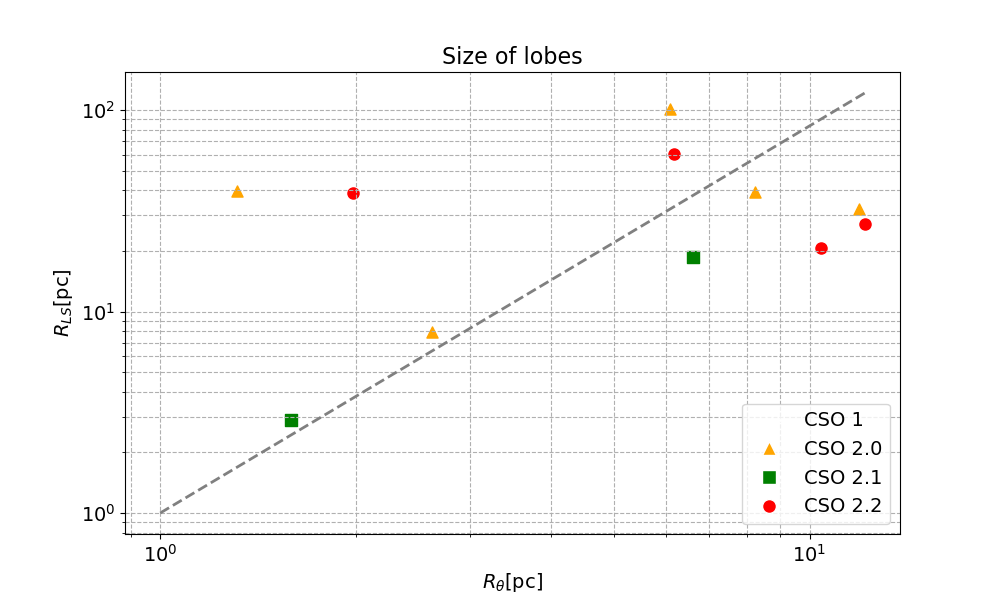
\includegraphics[width=0.8\textwidth]{C:/Users/henri/OneDrive/Documents/NTNU/Semester 10/Masteroppgave/Plots/Size_of_lobes.png}
    \caption{Size of the emitting region estimated from the FWHM of the Gaussian fit at $5$ GHz and the linear size of the source.}
    \label{fig:lobe_size}
\end{figure}

We can see clearly that the linear relation equation significantly increases the size of our emitting region. The method of scaling the linear size to estimate the lobe size as explained in \cite{W_jtowicz_2020} leaves a lot to be desired since the linear size encapulates the entire lobe, and not just the hotspot. The image of a hotspot following the bowshock as the lobe expands is a more compelling region of acceleration than the entire lobe, and we would argue that the hotspot size is what one really wants. There is a compelling place for the linear size estimate when we want to estimate the jet power of our sources. In this scenario we wish not only to know the size of the hotspot, but also the size of the entire lobe, since the entire lobe is interacting with the ambient medium.  

Ideally we would want to have a time variable estimate instead of a physical estimate of the hotspot size, due to it being a more accurate representation of the emission region. This however is not possible with the data we have. We would argue that observations of a full catalouge of bona fide CSOs over several years would be of great interest to the scientifc community, and would give a much clearer image of emission region in CSO lobes. 

The conclusion of this analysis is that the FWHM method is more reliable when we are looking for areas that can accelerate particles, and we will use this method for the continued work in this thesis if possible. The linear size relation will be used if we do not have the FWHM of the Gaussian fit in jet power estimations.

\section{Energy budget}
Via the energy budget of the CSOs, we can get an idea of where it is possible to accelerate protons to UHECR energies.

\subsection{Hillas criterion}

 The first check is in the Hillas diagram, where we can compare the size and magnetic field strength of the system to the Hillas criterion. From our magnetic field estimations, we can see that the magnetic field strength is between $10^{-2}$ and $1$ G using both methods, and for radius estimation our hot spot is on the order of $2$ pc to $10$ pc when using the FWHM estimation method. It would be reasonable to assume that as the lobe expands, the magnetic field strength decreases, but as it expands, more energy is also being fed into the hotspots. Therefore, we can assume a magnetic field strength of $10^{-1}$ G for the biggest lobes as well. The choice of magnetic field strength and radius of the emitting region can be compared to other candidates via the Hillas criterion and is shown in Figure \ref{fig:Hillas}.


\begin{figure}
    \centering
    \includegraphics[width=0.8\textwidth]{C:/Users/henri/OneDrive/Documents/NTNU/Semester 10/Masteroppgave/Plots/hillas.png}
    \caption{Hillas diagram for the CSO. The red line represents the maximum energy of the proton that can be accelerated in the system, and blue is the same just for Iron. Dotted line represents a less efficient acceleration }
    \label{fig:Hillas}
\end{figure}

%From the figure it becomes clearer that CSO is a class worthy of being investigated further, both their lobe size, and their magnetic field strength make them great candidates. As for all potential sources one observes one needs a highly efficient acceleration mechanism in order to accelerate the protons. The efficiency of acceleration is described by the $\beta$ factor in figure \ref*{fig:Hillas}. The CSO hotspots separate themselves from usual AGN hotspots which are attributed to large lobes at the end of the jet in huge radio galaxies. The more compact hotspots in CSOs might be more efficient in accelerating protons, but this needs to be looked into further.  
%\section{x-ray power}
%In stduies such as \cite{Jacobsen:2015mga} and \cite{10.1111/j.1745-3933.2008.00499.x} one discuss the possibility of using the x-ray flux or hard x-ray flux as a proxy for hadronic acceleration. This is a common start in trying to probe the biggest emitters of neutrinoes and UHECRs, and it is worth looking at CSOs this way as well. The biggest caveat with this method is that one usually attributes the x-ray flux to the core region, and then one might have different mechanisms for acceleration than one has in the hotspots. In the case of our model of a CSO SED one immeditly sees that the total x-ray flux from the x-ray corona will be a factor of the total accretion luminosity. For our model of timescales later in the chapter one assumes the fraction to be $f_X = 0.3$. and for this one recived a typical total x-ray corona flux of $3 \times 10^{42} $erg/s. This number is quite a lot higher than  what was found by  \cite{bronzini2024investigating} who using two spectral models, found a x-ray flux for two compact sources, PKS 1718-649 and TXS 1146+596, to be just shy of $10^{41}$ erg/s. In addition to this estimate \cite{W_jtowicz_2020} cites the x-ray flux of 17 CSOs and here one will do another cross correlation with the CSOs in table \ref*{tab:CSO_sources}. The results can be seen in table \ref{tab:CSO_xray}.
From figure \ref{fig:Hillas}, it becomes clearer that CSOs are a class worthy of being investigated further; both their lobe size and their magnetic field strength make them good candidates. The CSO hotspots separate themselves from usual AGN hotspots, which are attributed to large lobes at the end of the jet in huge radio galaxies by having higher B field but lower sizes. One sees that for protons in low beta factors the CSOs are not sufficient.   %The more compact hotspots in CSOs might be more efficient in accelerating protons, but this needs to be looked into further.

\subsection{X-ray power}
In studies such as \cite{Jacobsen:2015mga} and \cite{10.1111/j.1745-3933.2008.00499.x}, they discuss the possibility of using the X-ray flux or hard X-ray flux as a proxy for hadronic acceleration. This is a common start in trying to probe the biggest emitters of neutrinos and UHECRs, and it is worth looking at CSOs this way as well. The biggest caveat with this method is that one usually attributes the X-ray flux to the core region, which is not always the dominant X-ray source. In the case of our model of a CSO SED in section \ref{sec:non_core_photon_fields}, we immediately sees that the total X-ray flux from the X-ray corona will be a factor of the total accretion luminosity. Non core dominated flux is also in our model subdominant. For our model of timescales later in the chapter, one assumes the fraction to be $f_X = 0.3$ which is taken from \cite{Ghisellini_2009}, and for this, one received a typical total X-ray corona flux of $3 \times 10^{42}$ erg/s for an accretion luminosity of $10^{43}$ erg/s. .  This number is quite a lot higher than what was found by \cite{bronzini2024investigating}, who, using two spectral models, found an X-ray flux for two compact sources, PKS 1718-649 and TXS 1146+596, to be just shy of $10^{41}$ erg/s. In addition to this estimate, \cite{W_jtowicz_2020} cites the X-ray flux of 17 CSOs, and here one will do another cross-correlation with the catalogue of CSOs in table \ref*{tab:CSO_sources}. The results can be seen in table \ref{tab:CSO_xray}.


\begin{table}
    \centering
    \begin{tabular}{|c|c|c|c|}
        \hline
        \textbf{Name} & \textbf{z} & \textbf{Class} &   \textbf{$L_{\text{X-ray}}$} \\
        \hline

        

        J0111+3906 & 0.66847 & 2.0 & 70 \\
        J0119+3210 & 0.0602 & 2.2 & $<$1.0 \\
        J0713+4349 & 0.518 & 2.0 & 394 \\
        J1511+0518 & 0.084 & 2.0 & 30 \\
        J1939-6342 & 0.183 & 2.0 & 6 \\
        J1944+5448 & 0.263 & 2.0 & 7.31 \\
        J1945+7055 & 0.101 & 2.2 & 12 \\ 
        J2022+6136& 0.227 & 2.1 & 112 \\
        J2355+4950 & 0.238 & 2.2 & 13 \\
        \hline
    \end{tabular}
    \caption{X-ray flux of the CSOs in table \ref{tab:CSO_sources} found in the data set in \cite{W_jtowicz_2020}. The X-flux is given in units of $10^{42}$ erg/s.}
\label{tab:CSO_xray}
\end{table}


After cross-correlation, we are left with $9$ objects that are in both catalogues. The X-ray flux of these objects spans the range between $6-394 \times 10^{42}$ erg/s for CSO $2.0$, which has the most data. CSO 2.2, with three data points, does not have any that exceed $13 \times 10^{42}$ erg/s, and the lone CSO $2.1$ sits at a powerful $112 \times 10^{42}$ erg/s. With these values, we can see how they compare to other AGN like BL Lacs and blazars. We will do this by looking at the total X-ray emissivity of the sources and comparing it to the local emissivity of the UHECRs and the total emissivity of neutrinos. The total X-ray emissivity is given by $Q_{\text{X-ray}} = L_{\text{X-ray}} n_{\text{CSO}}$. Here the density applied is the theoretical we calculated in section \ref{sec:prevalence} at $1.2 \times 10^{-5} $$\text{Mpc}^{-3}$. The results can be seen in figure \ref{fig:X-ray_em}. 

The amount of data collected is quite low, and we cannot make any strong conclusions from this, but using the values as a benchmark, we can see that the X-ray emissivity of the CSO $2.0$ and $2.1$ spans a sizeable area above the emissivity of UHECRs and neutrinos. CSO $2.2$ seems to emit X-ray at a lower rate but still powerful enough to exceed the local emissivity of UHECRs. I have found that even though the X-ray flux is a good indicator of relativistic particles, in most cases electrons, there still is work to be done relating it to UHECRs and neutrinos. Given that the X-ray flux of the CSOs surpasses the local emissivity of UHECRs and neutrinos significantly, we can say that the CSOs are also good candidates for UHECRs and neutrino production when compared to other AGN classes.



\begin{figure}[H]
    
    \centering
    \begin{subfigure}[b]{0.49\textwidth}
        \centering
        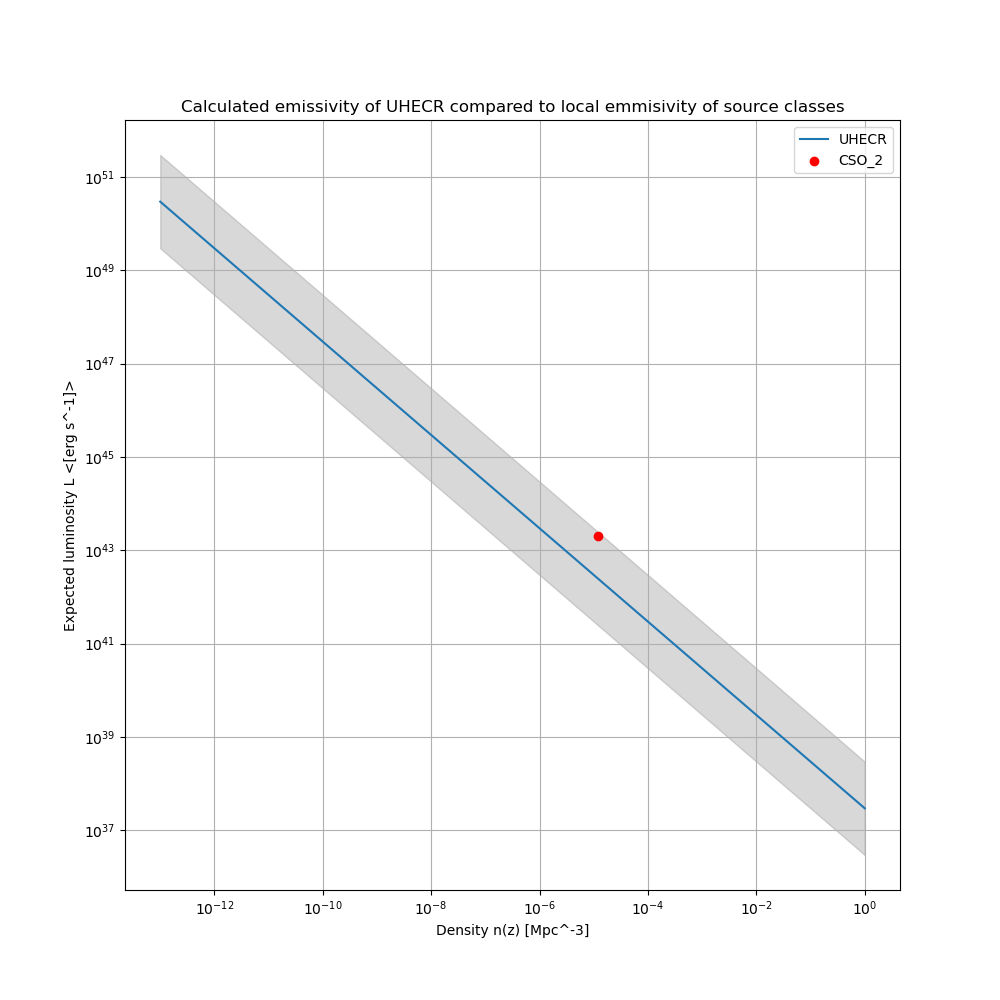
\includegraphics[width=\textwidth]{C:/Users/henri/OneDrive/Documents/NTNU/Semester 10/Masteroppgave/Plots/L_n_uhecr_calc_cso.png}
        %\caption{UHECRs emissivity compared to X-ray luminosity of 
       
        %\label{fig:uhecr_em}
    \end{subfigure}
    \hfill
    \begin{subfigure}[b]{0.49\textwidth}
        \centering
        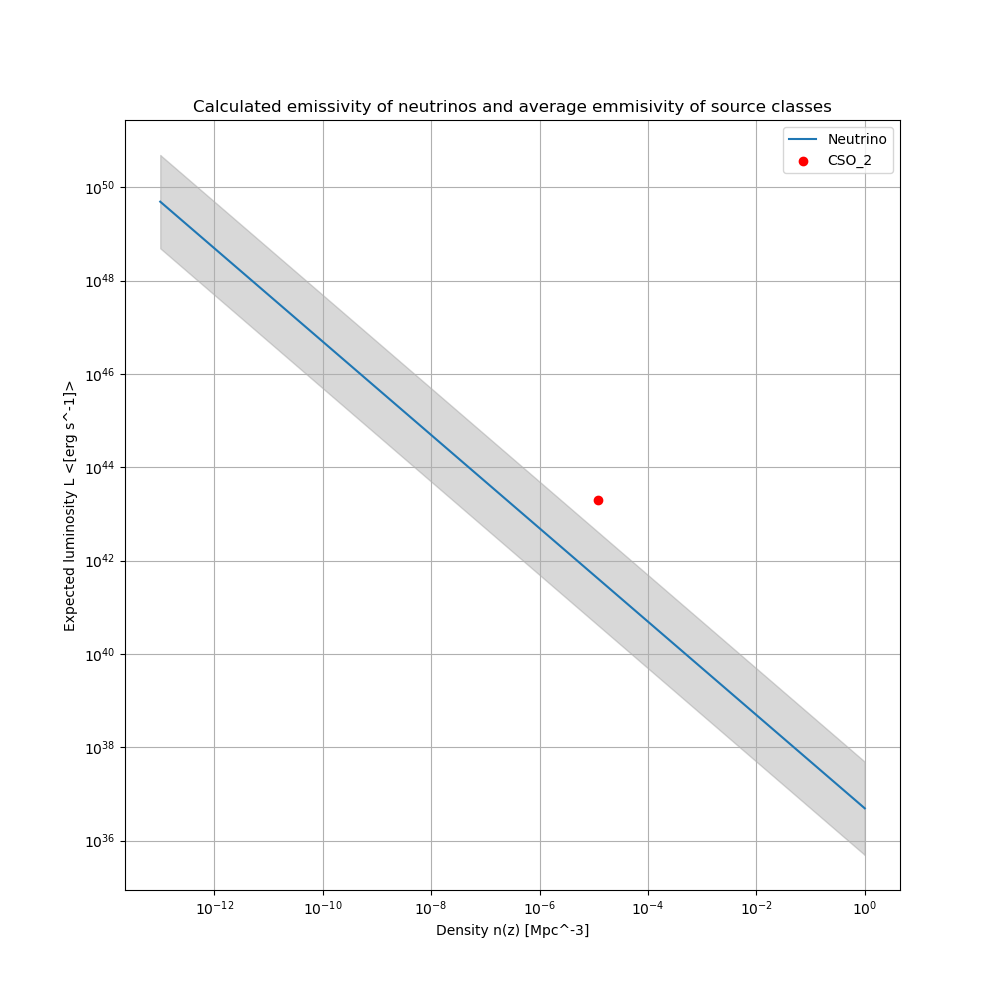
\includegraphics[width=\textwidth]{C:/Users/henri/OneDrive/Documents/NTNU/Semester 10/Masteroppgave/Plots/L_n_neut_calc_cso.png}
        %\caption{Neutrinos emissivity compared to X-ray luminosity of AGN classes}
        %\label{fig:neut_em}
    \end{subfigure}
    \caption{X-ray emissivity of CSO classes compared to local emissivity of UHECRs and neutrinos.}
    \label{fig:X-ray_em}
\end{figure}


%\section{Radio power}



\subsection{Jet power}

The jet power of jetted AGN is an important parameter in constraining parameters such as particle energy density, and radiative efficiency. If the jet energy is carried by particles, one can relate the comoving particle density to the stationary frame jet power $P_j$ as,

\begin{equation}
    \frac{P_j}{2\Omega_j R^2 c \beta (\Gamma m_e c^2)} = \Gamma n
\end{equation}

This is for a two-sided jet, where $\Omega_j$ is the jet opening angle in sr. The jet power relation here includes the assumption that the jet is carried by electrons and that the jet power is related to the bulk Lorentz factor of the plasma outflow. By using a general particle distribution for electrons, for example, as seen in equation \ref{eq:proton_spectrum} and including a factor to account for kinetic energy being carried by protons, we can represent the jet power as a function of the kinetic energy carried by particles. We add to this the power required to expel magnetic field-laden plasma given as

\begin{equation}
    P_b = 2 \frac{B^2}{8\pi} \Omega_j R^2 c \beta \Gamma^2
\end{equation}

By now including the equipartition magnetic field $B_{\text{eq}}$ and rewriting the kinetic terms as done in section \ref{sec:equipartition}, We can relate the minimum jet power as a function of the equipartition magnetic field. We are skipping a few steps of derivation, but this can be found in \cite{BHradiation} on page 136. The result is the minimum jet power of the system as a function of the equipartition magnetic field strength given as

\begin{equation}
    P_j(B_{\text{min}}) = \frac{98}{25}\pi c \beta \Gamma^2 r_b^2 \frac{B_{\text{eq}}^2}{8 \pi}
\end{equation}

Here we have used the equivalence $B_{\text{min}} = 0.92 B_{\text{eq}}$, and$r_b= \frac{R_{\text{eff}}}{3^{1/3}}$ is the transverse width of the jet. 


The last quantities that need to be estimated are the bulk Lorentz factor and, importantly, jet $\beta$, or the speed of expansion into the surrounding medium. The bulk Lorentz factor of our jet is estimated to be $\Gamma < 1.1$ since CSO jets are not relativistically beamed. The last value is the expansion speed of the jet, which will vary from class to class. In the case of CSO $2.0$, one will estimate a value of $\beta$ between $0.1 - 0.4$ c. In \cite{sullivan2024smallscale}, they cite the expansion speed of a CSO $2.0$ to be approximately $200 \times c_s = 200 \times 250$ km/s, where $c_s$ is the sound speed. This gives a value of $\beta = 0.166$ c. Part of the definition of CSO $2.1$ is that the jet is decelerating, and therefore one would expect $\beta$ to lie between $0.1$ and $8\times 10^{-4}$ c. Lastly, the speed of the jet in CSO $2.2$ is by definition extremely low or non-existent, where the apparent motion of emitting bubbles is due to adiabatic expansion. Therefore, one argues that the speed of any emitting blob is to move at the speed of sound in the medium, and therefore $\beta = 8\times 10^{-4}$ c. %For values of jet energy derived this way, one will argue that they mostly will work for CSO $2.0$ due to the fact that their jet opening angle has not evolved greatly from their initial state.

One will need to compare this jet power to another method in order to investigate the underlying dynamics. In \cite{Broderick_2015}, one finds a relation between the jet power and the accretion rate of the system. The relation is given as

\begin{equation}
    P_j = \eta_j \dot{M} c^2
\end{equation}

where $\eta_j$ is an efficiency constant . One can estimate the accretion rate as a fraction of the X-ray luminosity via some simple assumptions. Like our broadband SED modeling, one assumes that the X-ray luminosity is a fraction of our accretion luminosity $L_{\text{X-ray}} = f_X L_{\text{d}}$. The accretion rate is given as $L_{\text{d}} = \eta_d \dot{M} c^2$ where $\eta_d$ is the efficiency of the accretion disk. By substituting the mass accretion rate as a function of the X-ray luminosity, one can get a simple estimate for the jet power. The resulting jet power is given as

\begin{equation}
    \label{eq:jet_power}
    P_j = \frac{\eta_j}{\eta_d f_X} L_{\text{X-ray}} = \alpha L_{\text{X-ray}}
\end{equation}

Here, $\alpha$ is a constant that absorbs the other constants since they are most likely dependent on each other. One also has from \cite{Broderick_2015} that $\eta_j < \eta_d$ and with a given disk efficiency of $\eta_d = 0.1$ one can estimate the ranges of $\alpha$. In \cite{W_jtowicz_2020} they estimate efficiency values of the order $0.001 \rightarrow 0.1$ for the jet, and in our model of the SED one assumes the value $f_X = 0.3$. Therefore, the range of $\alpha$ can be estimated to lie between $0.03 \rightarrow 3$. One will utilize the table \ref{tab:CSO_xray} to estimate the jet power of the CSOs, but one needs to define the equipartition magnetic field for them as well. Since one does not have NRAO data for these sources, one will use the relation between linear size and radius to estimate the radius of the lobes. Otherwise, the flux density $S_v$ is given in \cite{W_jtowicz_2020} with the corresponding X-ray luminosity. The jet power from the two methods can then be seen in Figure \ref{fig:jet_power}.


\begin{figure}
    \centering
    \includegraphics[width=0.8\textwidth]{C:/Users/henri/OneDrive/Documents/NTNU/Semester 10/Masteroppgave/Plots/jet_power.png}
    \caption{Jet power of the CSOs in table \ref{tab:CSO_sources} via two methods. The jet power is calculated using the minimum jet power argument based on magnetic field equipartition and using the x-ray luminosity as a proxy. The errorbars for minimum jet power are calculated from the span of values obtained from different $\beta$ values and the errorbars for x-ray luminosity are calculated from the span of values obtained from different $\alpha$ values.} 
    \label{fig:jet_power}
\end{figure}

The figure shows that the jet power estimated from the X-ray luminosity is significantly lower for CSO $2.0$ and $2.1$ than the minimum jet power estimated from the equipartition magnetic field and vice versa for CSO $2.2$. The values obtained through the equipartion argument are very large, but remain in the domain of other jetted FR II galaxies as seen in \cite{Godfrey2013}. The reason for the large value might be the overestimation of the lobe size which will lead to an overestimation of the jet power. The x-ray inferred power seems to give more reasonable number since \cite{readhead2023compact} found the jet power of CSO to reach values of $10^{44}$ erg/s, which is in the same order of magnitude as the most powerfull CSO in our sample.


With more constrained jet power one could investigate the required proton content of the sources. It would be interesting to have more concrete data directly measuring the jet power of specific CSOs. This would give us a more concrete value of the jet power and allow us to make bolder claims on the necessaty of protons in the lobes.
By folllwing the reasoning as done in \cite{Wykes_2013} the results as they stand do not require protons in the lobes to explain the jet power, but this result still bears a significant amount of uncertainty.  




\section{Characteristic timescales in CSO hotspots}

Looking at characteristic timescales for CSOs is a powerful tool for understanding the maximum energy that can be obtained from the system. In section 4, we outlined the general method, and here we will present the results for CSO 2s. The equations for the timescales are given in section \ref{sec:time_scales}.
With the given data obtained from measurements, we will define conservative estimates for an acceleration region in the CSO. The regions of interest are the hotspots created during the CSO $2.0$ and $2.1$ stages, and we will observe that these are good regions for acceleration. The first constant that needs to be estimated is the size of our emitting system. From observations, it is clear that the radio lobes expand significantly during the CSO lifetime. From radio variations made by \cite{bronzini2024investigating} they find a Radio variation on the order of tens of years which relates to a size estimate of approximately $2$pc. Additionally our result from earler sections indicate a source size between $1-10$ pc. Therefore,  a reasonably conservative estimate for the size of the lobes is $R_{\text{lobe}} = 2$ pc. In addition to this size requirement, we will also include the lifetime of the source, which is on the order of $10^3$ years for comparisson.

\begin{figure}
    \centering
    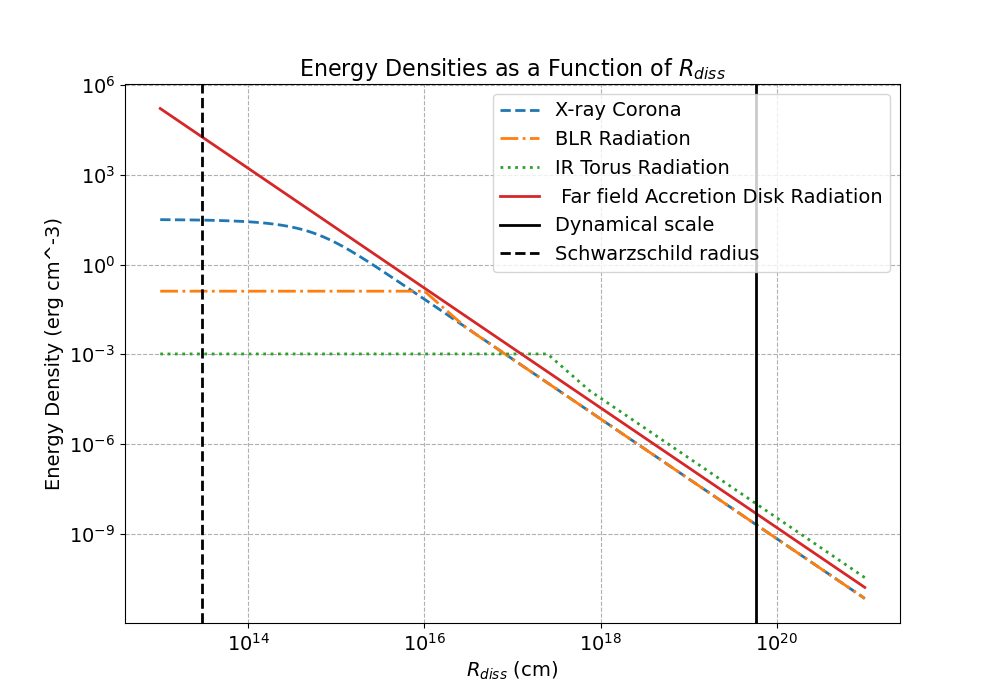
\includegraphics[width=0.8\textwidth]{C:/Users/henri/OneDrive/Documents/NTNU/Semester 10/Masteroppgave/Plots/Energy_densities.png}
    \caption{The energy density of the different photon fields created by the different regions in the CSO as a function of distance.}
    \label{fig:energy_densities}
\end{figure}

In estimating the magnetic field strength, we found the values of typical lobes to be $B \ge 10^{-2}$ G from the equipartition argument. This value is a reasonable lower limit for the magnetic field strength. It is important to note that the magnetic field strength is a very important parameter and yet bears significant uncertainty. 

For the photopion production, one will use the photon field as described in section 4, where the used parameters can be found in table \ref{tab:SED_params} with corresponding source. This field is based on the field of a much larger AGN, but one assumes for this discussion that the field is similar in the CSO. One can compare this generated field to the ones presented in \cite{bronzini2024investigating}, where they find a similar magnitude and shape of the resulting SED. A significant note is that the field is also not strongly beamed, giving room for other parts of AGNs to be seen. The resulting energy densities is seen in figure \ref{fig:SED_sep}. The exact shape of the energy densities is not incredibly important for the following discussion, but the broad shape and magnitude are important. The exact shape will become more important when one starts looking for observational signatures of the acceleration, such as gamma rays, and here one can use the model and minimize the parameter space to find the best fit. The energy densities of the photon fields is scaled to incorparete the distance of the hotspot from the core. This distance is set to $D = 5$pc and the energy densities are scaled as seen in figure \ref{fig:energy_densities}.  


\begin{figure}
    \centering
    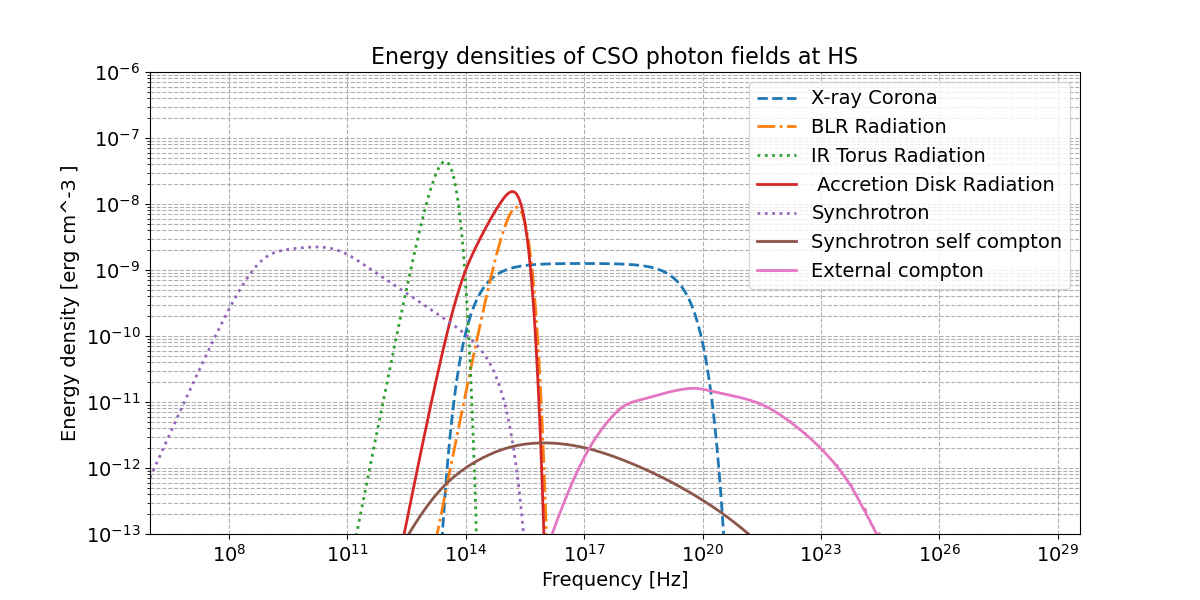
\includegraphics[width=1\textwidth]{C:/Users/henri/OneDrive/Documents/NTNU/Semester 10/Masteroppgave/Plots/SEDs_sep.png}
    \caption{Energy density of the different emitting regions of a CSO as seen by the hotspot. The SED is based on the parameters in table \ref{tab:SED_params}.}
    \label{fig:SED_sep}
\end{figure}






\begin{table}
    \centering
    \begin{tabular}{|c|c|c|}
        \hline
        Parameter & Value & Source \\
        \hline
        $L_{d}$ & $10^{43}$ erg/s & [2] \\
        $GM$ & $G 10^{8} M_{\odot}$ &[3]\\
        $RS$ & $\frac{2GM}{c^2}$ & - \\
        $\eta$ & 0.1 & [1]\\
        $f_{X}$ & 0.3 & [1]\\
        $R_{X}$ & 30$ RS $ & [1]\\
        $\beta$ & 0.4 $c$ &[4]\\
        $f_{\text{BLR}}$ & 0.1  &[1]\\
        $R_{\text{BLR}}$ & $10^{17} \sqrt{L_{d}/10^{45}}$ cm &[1]\\
        $f_{\text{IR}}$ & 0.5&[1] \\
        $R_{\text{IR}}$ & $2.5 10^{18}\sqrt{L_{d}/10^{45}}$ cm &[1] \\
        $\Gamma$ & 1.1 & -\\
        $T_{\text{IR}} $ & $ 370$ K &[1]\\ 
        $\nu_{BLR}^{\text{peak}} $ & $ 2.47 10^{15}$ Hz  & [1]\\
        $\gamma_{\text{min}} - \gamma_{\text{max}}$ & $1 - 10^5$ & [5]\\ 
        \hline
    \end{tabular}
    \caption{Parameters used to determine the SED of the different regions.The sources for the parameters are as follow; [1] \cite{Ghisellini_2009}, [2] \cite{bronzini2024investigating}, [3] \cite{W_jtowicz_2020}, [4] \cite{sullivan2024smallscale}, [5] \cite{BHradiation}.}
    \label{tab:SED_params}
\end{table}


From the above parameters one can estimate the characteristic timescales for the CSO, seen in figure \ref{fig:timescales}. 

The timescales show us that high-energy protons can, and in any case will, under the right conditions, accelerate up to energies of $<10^{20}$ eV. This limit is capped by the dynamical size of the emitting region and, of course, the magnetic field strength. The timescales also show us that the acceleration is dominated by synchrotron losses and photopion losses, and due to their small value, one would need to consider pair-pair losses as well, which is not done in this analysis. The lack of photopion loss dominance is a good sign for proton acceleration since it has been a limiting factor in other studies such as \cite{peretti2023diffusive}, where one has a higher luminosity object with processes happening even closer to the central engine. One can confirm the lack of photopion by comparing it to the work of \cite{TAKAMI2011749}, which considered a young radio AGN with much bigger lobe sizes and much higher luminosity, but got similar results. The lack of photopion interaction will also be a limiting factor for neutrino production, something that will be discussed in the following sections.

\begin{figure}[H]
    \centering
    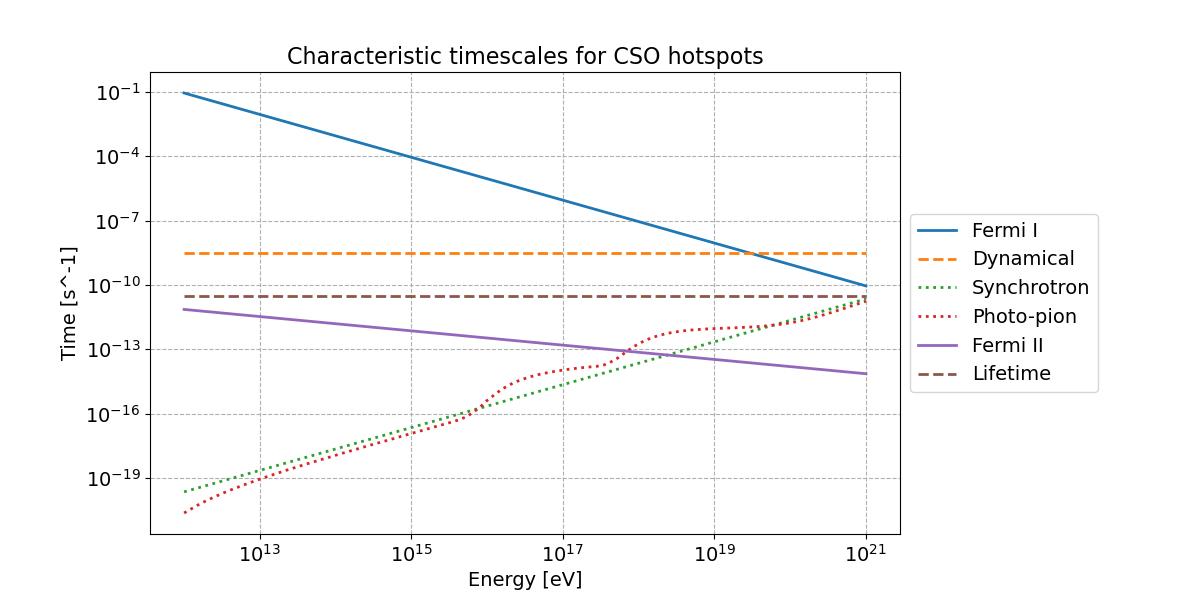
\includegraphics[width=1\textwidth]{C:/Users/henri/OneDrive/Documents/NTNU/Semester 10/Masteroppgave/Plots/Time_scales.png}
    \caption{Characteristic timescales for the CSO. Processes included is synchrotron losses and photopion losses. The timescales are calculated for a spherical size of $R_{\text{lobe}} = 2 pc$ and a magnetic field strength of $B = 10^{-2} G$. The photon field is based on the parameters in table \ref{tab:SED_params}.}
    \label{fig:timescales}
\end{figure}

%\section*{Acceleration}
From the above timescales, one can see that the maximum energy that can be obtained from the system via first-order Fermi acceleration is huge and significantly larger compared to second-order acceleration. For CSOs to remain candidates, it is clear that only first-order acceleration is possible, and therefore one will only consider this. One can justify that first-order acceleration happens in the hot spot due to the expansion of the lobes into the ambient medium. From radio observations, and the discussion in the previous section CSOs have measured mildly relativistic expansion of the lobes, and with this comes naturally a shock boundary between the expanding hot spot and the ambient medium. This shock boundary produces a natural place for acceleration. One can view the theoretical schematic of the shock in figure \ref{fig:CSO_shock}.

Second-order Fermi acceleration is not efficient in the CSO, which was to be expected. The acceleration is limited by the small size of the system, the low magnetic field strength, the assumed too-high proton density which was $n=10^{-4}$, which leads to a low Alfvén wave speed, and more. One would need a substantial decrease in the acceleration timescale for second-order acceleration to be efficient. This is not the case in the CSO, and one can therefore estimate that the acceleration is dominated by first-order acceleration.

\begin{figure}[H]
    \centering
    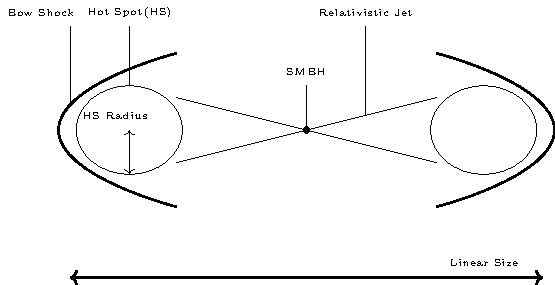
\includegraphics[width=0.5\textwidth]{C:/Users/henri/OneDrive/Documents/NTNU/Semester 10/Masteroppgave/Plots/Expansion_of_lobes.pdf}
    \caption{Schematic of the shock in the CSO. The shock is created by the expansion of the lobes into the ambient medium through jet pressure. Image inspired from \cite{Perucho_2002}}
    \label{fig:CSO_shock}
\end{figure}


\section{Discussion}
The results presented indicate that CSOs hotspots are promising candidates in the search for natural particle accelerators. The magnetic field strength and the size of the emitting region are of the appropriate order of magnitude, suggesting that these objects have the necessary conditions to support high-energy processes. Additionally, the presence of high jet powers in CSOs can implies that a substantial fraction of jet energy could be used in the acceleration of particles. 

Furthermore, the analysis of timescales reveals that the maximum energy attainable from the system via first-order Fermi acceleration is below $10^{20}$eV. This is a positive finding, as it provides a constraint on the potential energy gains within these environments. Moreover, the lack of photopion losses, which would otherwise lead to significant energy losses, is an encouraging sign. It suggests that the particles can retain most of their energy during the acceleration process, thereby making CSOs quite efficient accelerators.

These combined factors of appropriate magnetic field strengths, sizable emitting regions, necessary energy sinks for deceleration, feasible maximum energy thresholds, and minimal energy loss through photopion processes collectively make CSOs strong candidates and warrant further investigation. The results in this chapter will be used in the following chapter to try and constrain particle production in the CSO hotspots.